
\chapter{Model systemu rekomendacyjnego chroniącego prywatność}

W rozdziale zaproponowanie rozwiązania zwiększającego bezpieczeństwo oraz zachowanie prywatnych danych użytkownika. W tym celu wykorzystano \textit{Federated learning} omówiony w rozdziale \ref{section:federatedLearning} wraz z dodatkowymi zabezpieczeniami mającymi na celu zniwelować przedstawione problemy związane z tym rozwiązaniem. Także przedstawiono jak mógłby wyglądać proces przygotowania takiej metody dla nowo-powstałego systemu jak i dla już zaimplementowanego systemu z wykorzystaniem dostępnych bibliotek i technologii.

\section{Projekt rozwiązania}

W proponowanym rozwiązaniu wyróżniono trzech aktorów. Pierwszy z nich, zwykły użytkownik uczestniczy w normalnym przebiegu zaproponowanym w rozwiązaniu \textit{Federated learning}. Użytkownik na podstawie swoich danych poprawia otrzymany przez serwer model, następnie bez ujawniania swoich danych przekazuje dalej wyłącznie poprawiony przez siebie model.

Jednym z potencjalnych problemów może być założenie, że użytkownicy będą uczciwie uczestniczyć w całym omawianym procesie. Oznacza, to że użytkownik może zmniejszyć skuteczność modelu rekomendacji poprzez umieszczenie w nich niepoprawnych danych (niezgodnych z rzeczywistością). W przypadku pojedynczego użytkownika, który próbuje zakłócić pracę systemu istnieje mechanizm uśredniający otrzymane wyniki od wszystkich użytkowników. Jednak w przypadku zorganizowanego ataku z wielu kont wyłącznie normalizacja może nie być wystarczająca. W celu poradzenia sobie z tym problemem wprowadzono drugi typ aktora - użytkownik niezaufany, który ma możliwość wyłącznie otrzymania modelu od serwera głównego. Jest on wyłączony z usprawnienia udostępnianego modelu (nie wysyła on swoich rezultatów uczenia). Tego typu użytkownik po określonym czasie użytkowania systemu, ilości wystawionych ocen lub po odpowiednim procesie weryfikacyjnym może zostać przemianowany na zwykłego użytkownika uczestniczącego w procesie usprawniania wspólnego modelu.

Kolejnym problemem może być koszt nauki na systemach mobilnych. Niektórzy użytkownicy mogą posiadać słabszy sprzęt (zasoby sprzętowe czy bateria), który może uniemożliwić ponowne uczenie otrzymanego modelu na urządzeniu. W przypadku wolnego łącza lub jego braku, problemem może być pobieranie lub odesłanie modelu do głównego serwera. W tym celu użytkownik z ograniczonymi zasobami zostałby zmuszony do przesłania swoich zaszyfrowanych danych do serwera, tam wykorzystując właściwości szyfrowania homomorficznego model zostałby zaktualizowany, a rekomendacje przesłane do użytkownika.

\section{Fazy budowania systemu rekomendacyjnego}

Podczas implementacji systemu rekomendacyjnego wykorzystano typowy przepływ (przedstawiony na rysunku \ref{fig:rs_pipeline}) używany do tworzenia tego typu serwisów, który składa się z następujące pięć faz \cite{rs_in_real}:
\begin{itemize}
    \item wstępne przetwarzanie - na ten etap składają się czynności związane z transformacją danych do macierzy użytkownik-produkt oraz normalizacja w celu spłaszczenia wartości odstających (użytkownicy, którzy są nad wyraz pozytywni oraz negatywni w stosunku do dawania ocen),
    \item trenowanie - proces budowania modelu,
    \item optymalizacja hiper parametrów - wielokrotne trenowanie w celu dostrojenia parametrów w taki sposób, aby uzyskać jak najlepsze wyniki,
    \item przetwarzanie końcowe - sortowanie danych w celu uzyskania N najlepszych rekomendacji dla użytkownika, filtrowanie oraz wykluczenie wcześniej zakupionych lub negatywnie ocenionych przedmiotów,
    \item ewaluacja - testowanie stworzonego modelu poprzez ukrywanie/maskowanie ocen, a następnie użycie miar do ewaluacji (szczegółowo opisane w podrozdziale \ref{metryki}).
\end{itemize}{}

\begin{figure}
    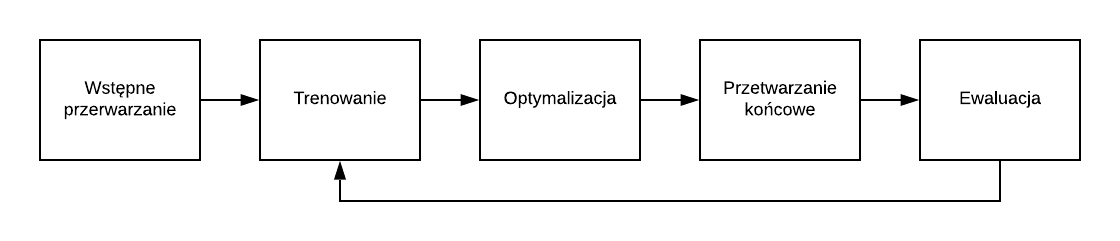
\includegraphics[scale=0.85]{rs_pipeline.png}
    \caption{Fazy przepływu podczas tworzenia systemu rekomendacyjnego.}
    \label{fig:rs_pipeline}
\end{figure}

\section{Dane testowe}

\section{Przegląd dostępnych technologii}

Istnieje wiele dostępnych bibliotek czy frameworków umożliwiające na implementacje rozwiązań typu \textit{Federated learning}. Większość z nich umożliwia na napisanie kodu w języku Python. Jednymi z bardziej popularnych oraz dobrze udokumentowanych są następujące technologie:

\begin{itemize}
    \item PySyft - narzędzie opracowane przez grupę OpenMinded. PySyft rozszerza popularne biblioteki takie jak: PyTorch, Tensorflow oraz Keras o możliwość zdalnego wykonywania, szyfrowania homomorficznego czy obliczenia z wykorzystaniem wielu użytkowników,
    \item Tensorflow Federated - biblioteka wykorzystywana do uczenia maszynowego i innych obliczeń na danych nie scentralizowanych oparta o otwarty kod źródłowy. Stworzona w celu badań oraz eksperymentowania z koncepcją \textit{Federated learning}.
\end{itemize}

\section{Fragmenty implementacji}
